\section{Master Thesis Proof of Concept Attempt (1 page)}
\label{section:initial_hexacopters}

In my master thesis~\cite{joshua_master_thesis}, I developed a method for fiducial precision landing with a gimbal-mounted camera.
The algorithm involves identifying fiducial markers through image analysis,
tracking the markers via a gimbal-mounted camera,
calculating position targets via coordinate system transforms in order to direct the drone towards the landing pad,
and communicating those position targets to the flight control software for approach.
I tested this algorithm in Gazebo simulator only, and the natural next step was to test it on a physical platform.
We have therefore built 2 Tarot 680 hexacopters,
which provides a good thrust-to-weight ratio,
and space for mounting multiple computational components.
A combination of Raspberry Pi 3B+ and Navio2~\cite{navio2_website} shield serve as a flight controller
that can communicate with a companion board.
The companion boards (a Google Coral Dev board and an NVIDIA Jetson Nano) communicate via Ethernet over USB to the flight
controller and perform all heavy computations involving image analysis, coordinate system transforms, PID control,
and position target generation.
Figure~\ref{figure:hardware_setup} outlines the hardware setup.

\begin{figure}
    \centering
    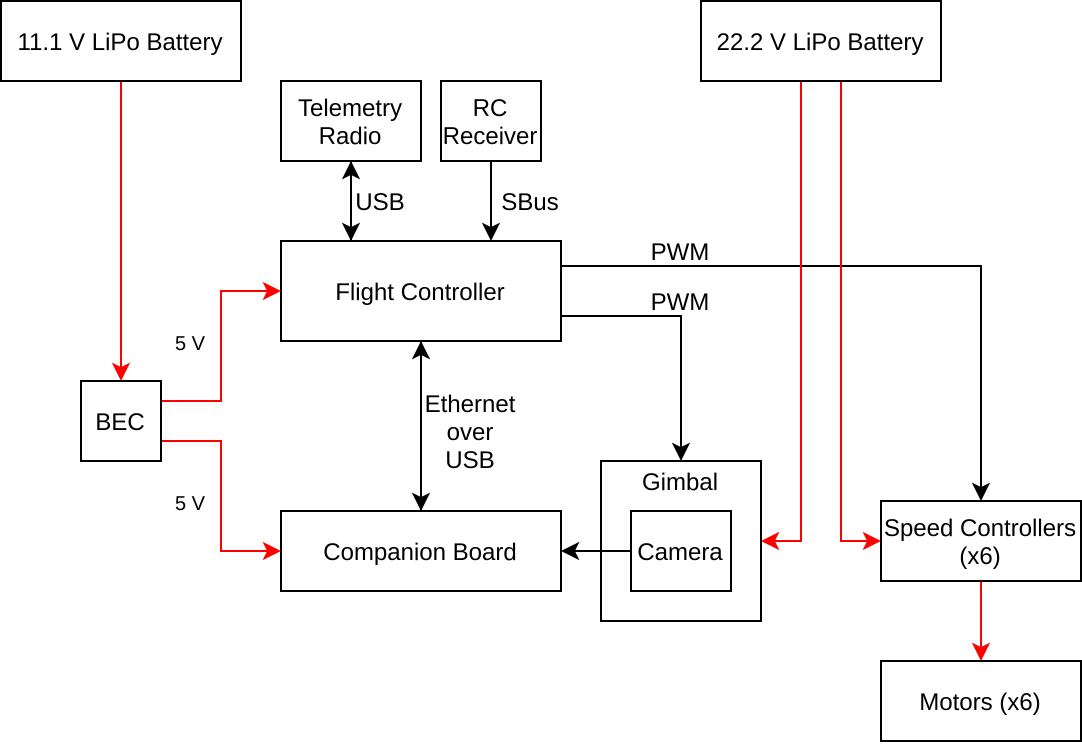
\includegraphics[width=0.6\textwidth]{images/hardware.png}
    \caption{Hardware Setup}
    \label{figure:hardware_setup}
\end{figure}

The computational components require some protection from the harsh Icelandic weather,
and we therefore designed and 3D-printed a component mounting plate with a connector for a canopy.
We also designed and printed cases to protect camera modules and allow them to be mounted in a gimbal with a GoPro form factor.
The fully assembled Jetson hexacopter are shown in Figure~\ref{figure:jetson_drone}.
(The Coral drone looks and performs similarly.)
The algorithm is implemented as a set of ROS modules.
A \texttt{gscam} node retrieves camera input and makes it available as a ROS topic,
after which a \texttt{whycon\_ros} node analyzes camera images to detect WhyCon/WhyCode markers and determine their pose.
A \texttt{gimbal\_controller} node reads the WhyCode detections, and passes the positions of the markers to 2 PID controllers,
which aim the gimbal tilt and pan in order to center the marker in the camera frame.
Finally, it passes the PID outputs as PWM signals to the gimbal.
A \texttt{landing\_controller} node reads the WhyCode detections,
performs coordinate system transforms to generate position targets,
and forwards them to the autopilot software.

\begin{figure}
    \centering
        \begin{subfigure}[b]{0.48\textwidth}
        \centering
        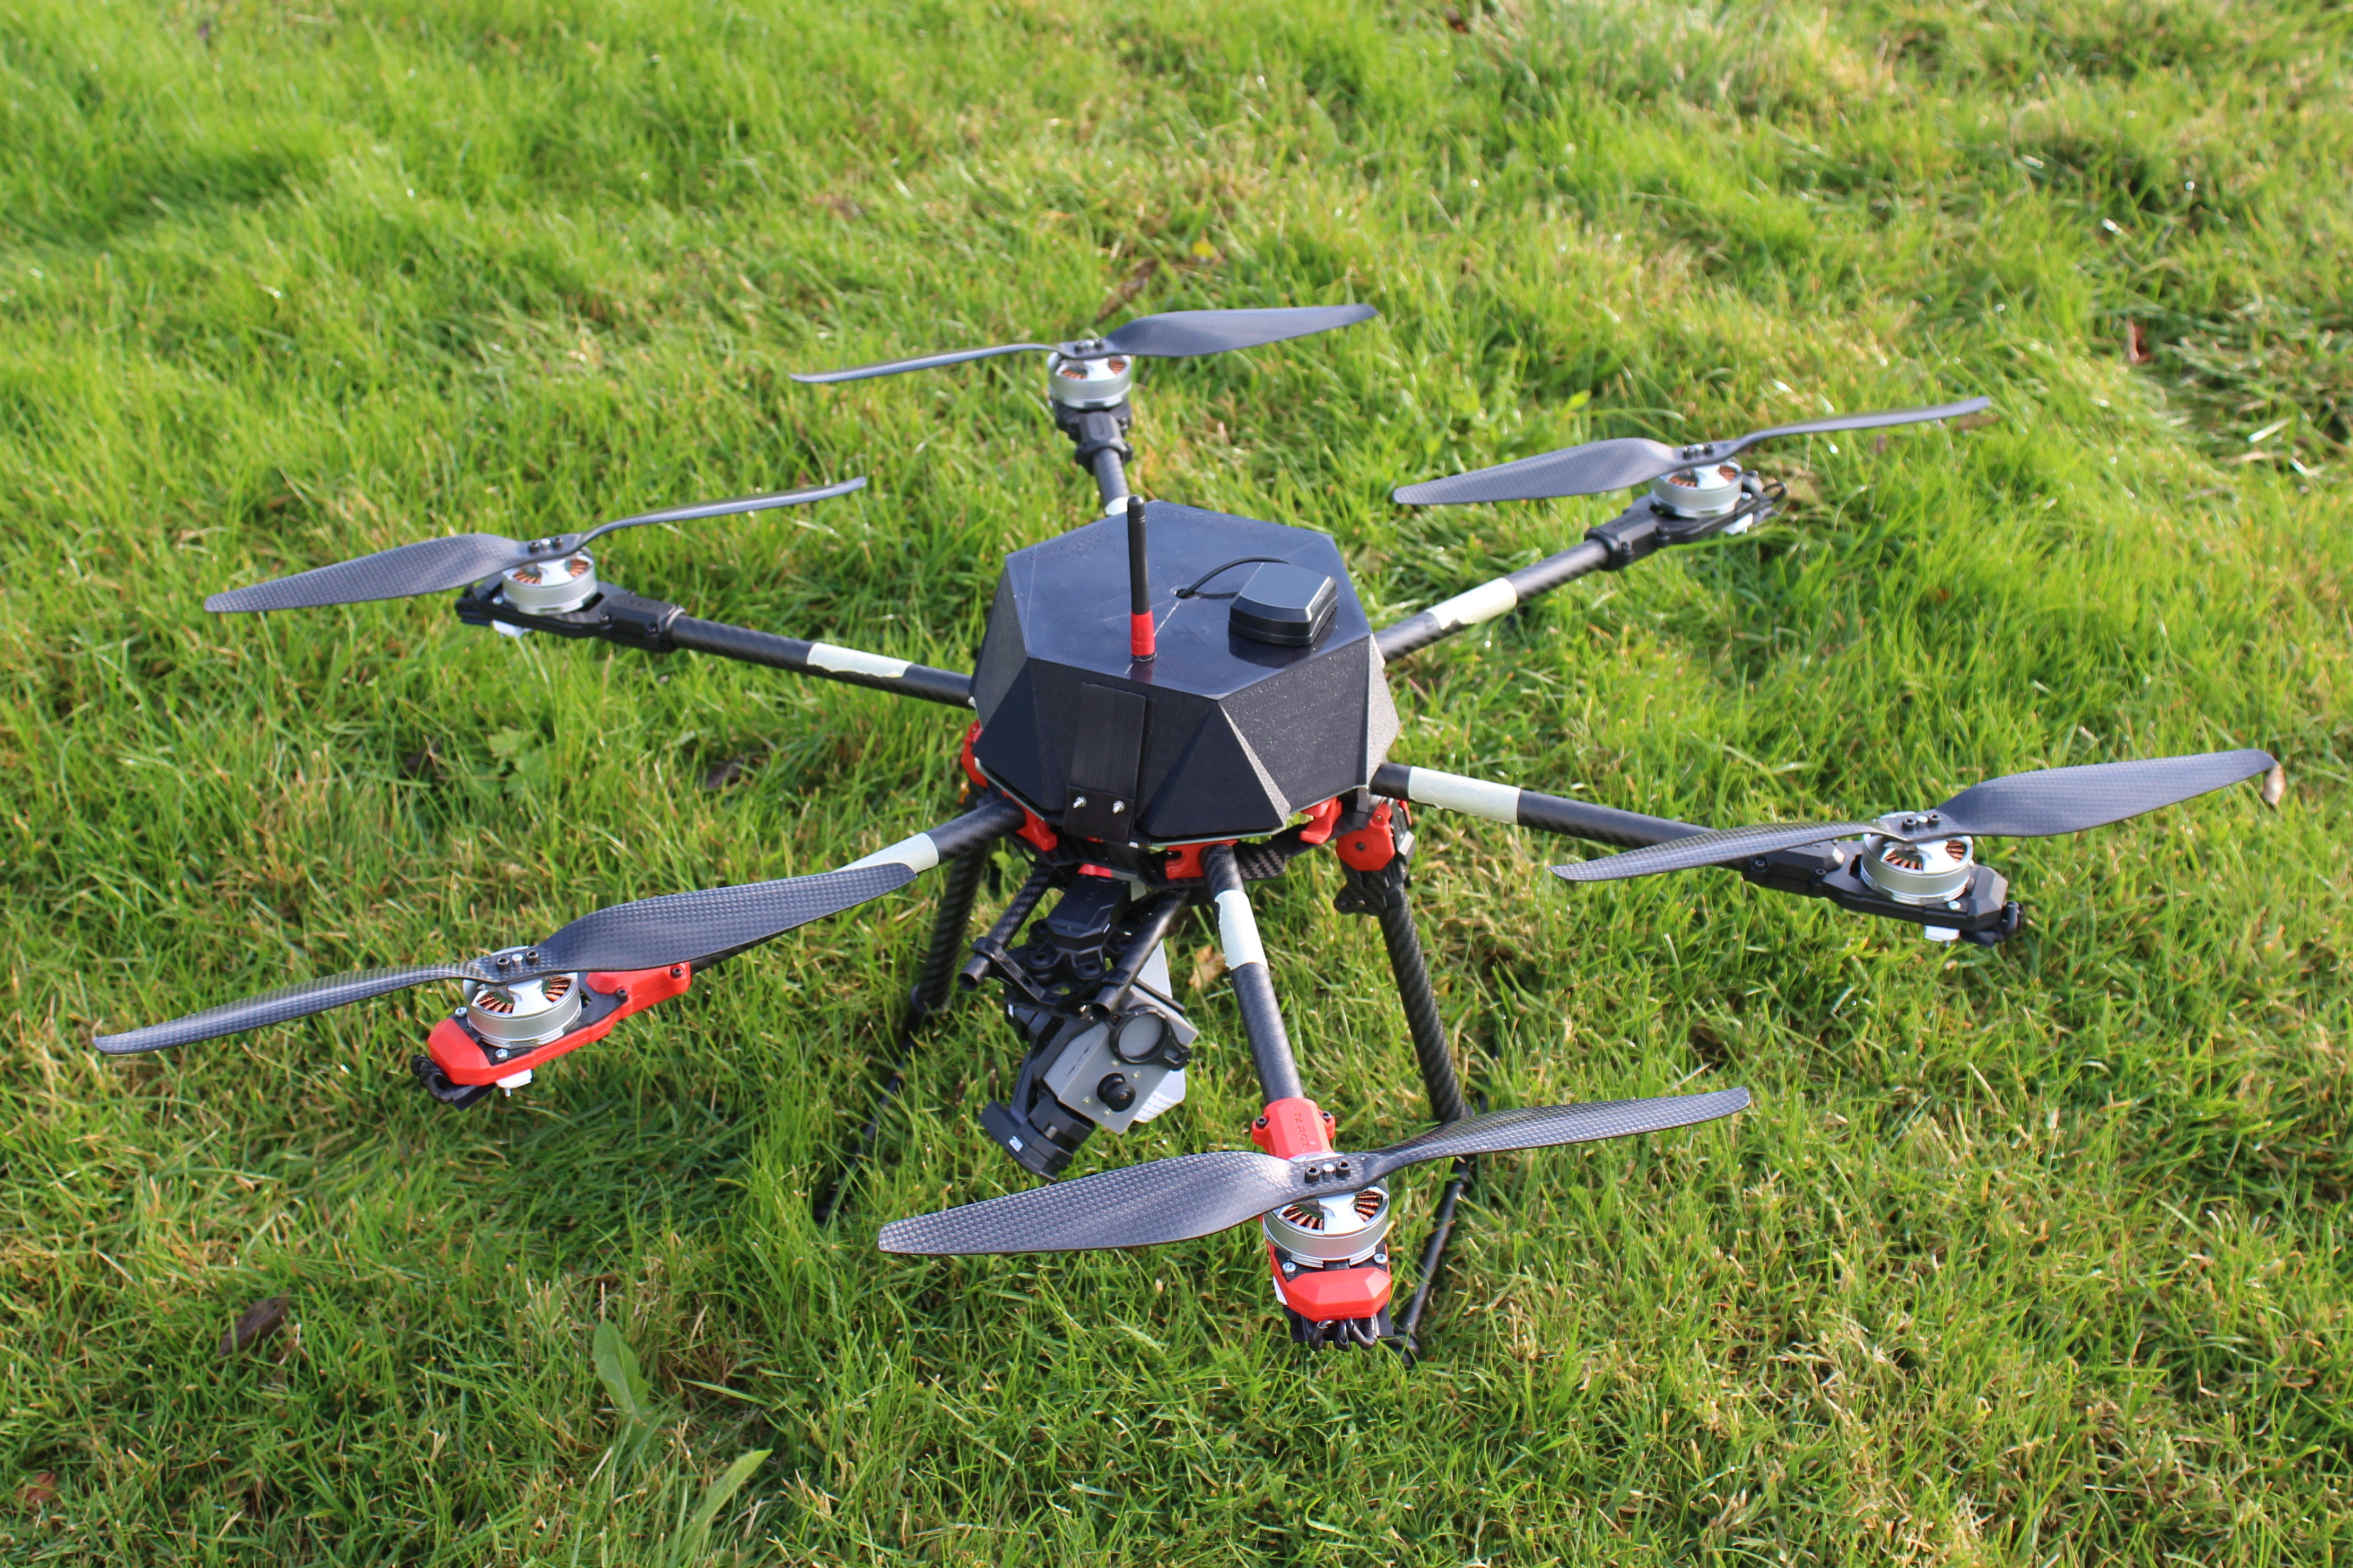
\includegraphics[width=\textwidth]{images/jetson_drone.JPG}
        \caption{The Jetson drone.}
        \label{figure:jetson_drone_external}
    \end{subfigure}
        \begin{subfigure}[b]{0.48\textwidth}
        \centering
        \includegraphics[width=\textwidth]{images/jetson_electronics.JPG}
        \caption{The Jetson drone's electronics compartment.}
        \label{figure:jetson_electronics}
    \end{subfigure}
    \begin{subfigure}[b]{0.49\textwidth}
        \centering
        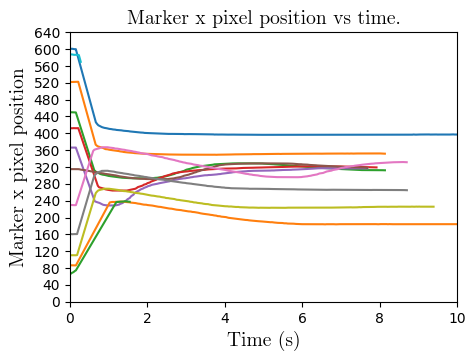
\includegraphics[width=\textwidth]{images/jetson_gimbal_performance_x_axis.png}
    \caption{Performance of the Jetson drone aiming the gimbal in the x axis.}
    \label{figure:jetson_gimbal_performance_x_axis}
    \end{subfigure}
    \begin{subfigure}[b]{0.49\textwidth}
        \centering
        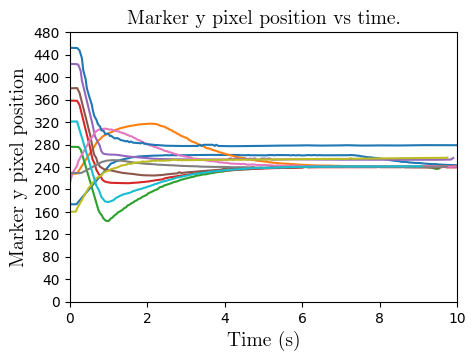
\includegraphics[width=\textwidth]{images/jetson_gimbal_performance_y_axis.png}
    \caption{Performance of the Jetson drone aiming the gimbal in the y axis.}
    \label{figure:jetson_gimbal_performance_y_axis}
    \end{subfigure}
    \caption{Performance of aiming the gimbal.}
    \label{figure:jetson_drone}
\end{figure}

\subsection{Results}

The drones fly with good stability even in high Icelandic winds, with an estimated 15-20 minute flight time.
\footnote{Video of some of the flights and landing attempts can be found at:
\href{https://vimeo.com/461576798}{https://vimeo.com/461576798}}
In lab tests and in flight, they are able to detect and track fiducial markers using the method
tested in simulation.
However, only the more lightweight WhyCon/WhyCode fiducial system was used in testing, instead of the
April Tag system, because of the time constraints of this summer project.
The performance of the drones in tracking the markers is shown in Figures~\ref{figure:jetson_gimbal_performance_x_axis}-\ref{figure:jetson_gimbal_performance_y_axis},
with the position of the marker in the camera frame in the given axis,
and with a resolution of 640x480 pixels after resizing in order to decrease the computational requirements
of the image analysis.
The wide angle lens of the Jetson Nano camera module results in much smoother tracking,
since each pixel corresponds to a larger distance than with the Google Coral camera module.

The drones are able to approach the landing pad autonomously,
but have not yet touched down autonomously.
This is due to two principal factors.
First, GPS precision is low in Iceland (i.e. geometric dilution of precision (GDOP) is relatively high)
because of Iceland's distance from the equator.
Methods of autonomous positioning within the ArduPilot framework which were not ostensibly GPS-based
are eventually translated into lat/lon/alt position targets,
and the drones attempted to navigate to them with GPS only (instead of other methods such as dead reckoning).
Since the GDOP was prohibitively high, the drones could not accurately estimate their position.
Therefore, they could only follow a coherent path for a limited amount of time when navigating autonomously,
after which the trajectory was unpredictable, even if the position target commands were correct.

Second, there is a fundamental challenge with fiducial markers
which comes as a result of the limitations of embedding 2-dimensional shapes into 3-dimensional spaces.
While the position of the marker in the camera frame can be detected unambiguously,
the orientation of the marker cannot.
Especially when the marker is almost normal to the camera's view,
its orientation becomes increasingly ambiguous in the roll and pitch components.
(This can be intuitively visualized by imagining the difference between the appearances of a marker
when it is at (roll,pitch,yaw)=$(1^{\circ}, 0, 0)$ versus $(-1^{\circ}, 0, 0)$.
These orientations would be difficult to distinguish even for the human eye, and much more difficult
for a camera with 640x480 pixels.)
Tests in simulation revealed this phenomenon, however, because of a variety of factors
(a more ``perfect'' camera/marker/world, better GPS, lack of logistical constraints, etc.),
this phenomenon was not prohibitive in simulation, and successful landings were plentiful.
These two problems set the stage for more research and modifications to the fiducial systems,
outlined in Section~\ref{section:fiducial_system_modifications}.